\section{MANUAL DE USUARIO}

En esta sección se va a describir como utilizar la aplicación generada en este trabajo.

Primero, al haber sido exportada a un ejecutable solo es necesario abrir el ejecutable, pero para que todo funcione es necesario que en la misma carpeta en la que se encuentra el ejecutable haya una 
carpeta con los recursos de la aplicación, que son:

\begin{itemize}
    \item Icono de la aplicación.
    \item Modelos de la red neuronal.
    \item Imágenes extra.
\end{itemize}

Estos elementos deberían venir en el \texttt{.zip} que contenga el ejecutable, si no están la aplicación no se abrirá.

Una vez abierta la aplicación, el usuario se encontrará con la ventana inicial de la \autoref{fig:ManualInicial}.
\begin{figure}[H]
    \centering
    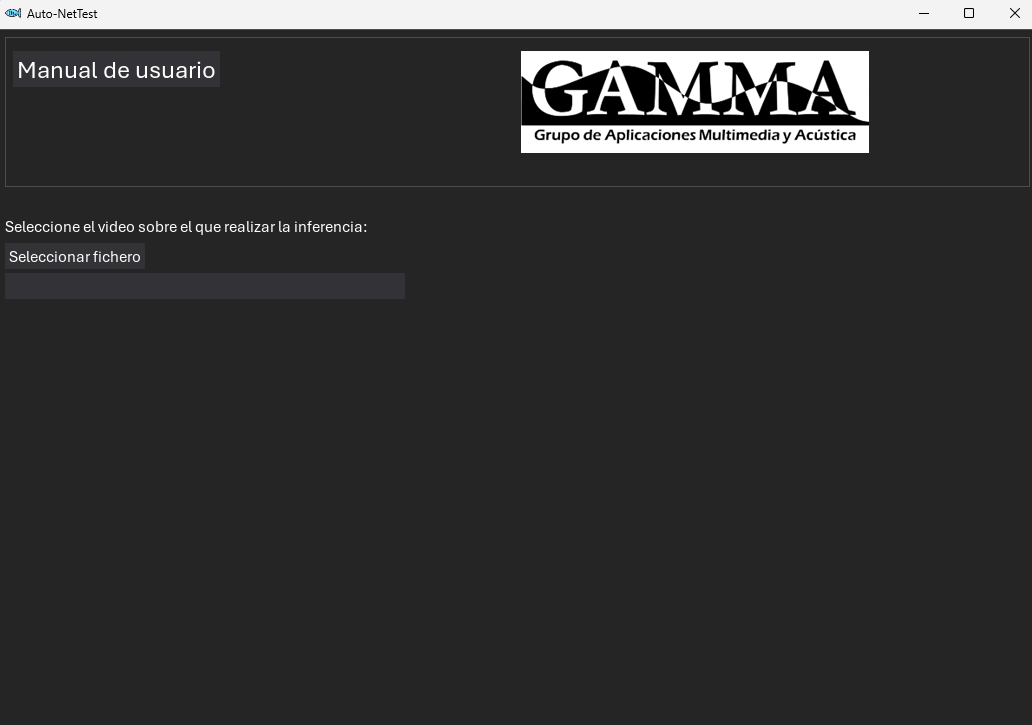
\includegraphics[width=0.9\textwidth]{images/9/Inicial.png}
    \caption{Ventana inicial de la aplicación}
    \label{fig:ManualInicial}
\end{figure}
En esta pantalla el usuario puede:
\begin{itemize}
    \item Abrir un manual propio en la aplicación que explica de forma resumida el funcionamiento de la misma.
    \item Seleccionar un video a través de un selector como se ve en la \autoref{fig:ExploradorManual}. Este selector está diseñado para que filtre los videos que tiene formato compatible con la aplicación, eso quiere decir 
    que sí el video no aparece, no es compatible y debe exportarse a otro formato.
    \begin{figure}[H]
        \centering
        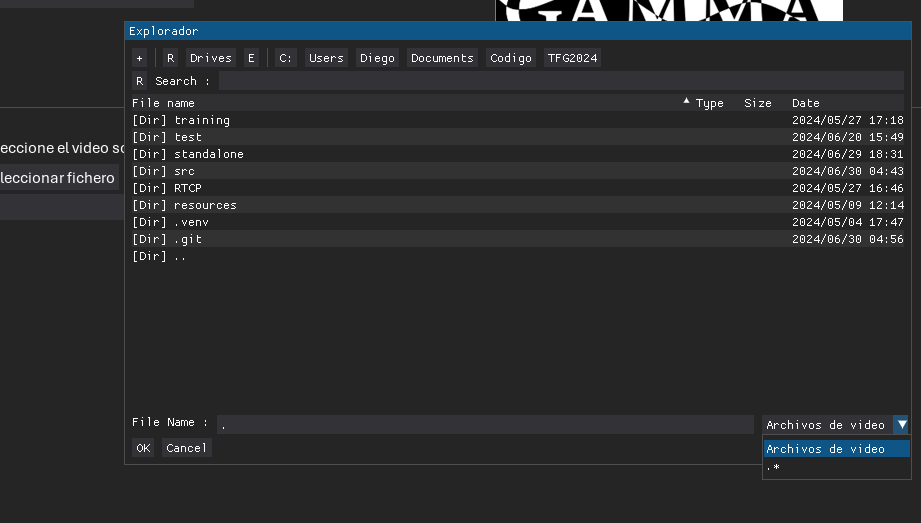
\includegraphics[width=0.9\textwidth]{images/9/Explorador.png}
        \caption{Vista del explorador para seleccionar video}
        \label{fig:ExploradorManual}
    \end{figure}
    \item Inferir: una vez seleccionado un video aparece un botón como el de la \autoref{fig:BotonInferirManual}. Una vez pulsado se hacen una serie de comprobaciones para que no haya ningún error y se pasa a la pestaña de carga.
    \begin{figure}[H]
        \centering
        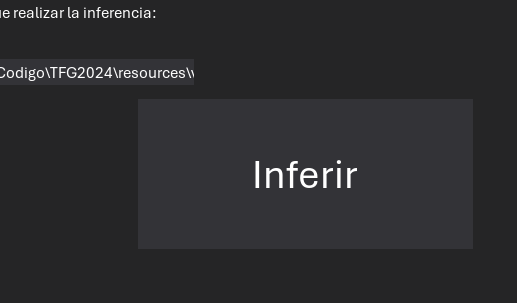
\includegraphics[width=0.9\textwidth]{images/9/InferirBoton.png}
        \caption{Botón de inferir de la ventana inicial de la aplicación}
        \label{fig:BotonInferirManual}
    \end{figure}
\end{itemize}
\clearpage
Una vez en la pantalla de carga, la cual se puede ver en la \autoref{fig:CargaParaManual}, el usuario puede observar el progreso en tiempo real del procesado del video. Además de esto, el usuario puede cancelar la inferencia con un 
botón que le devuelve a la ventana principal.

\begin{figure}[H]
    \centering
    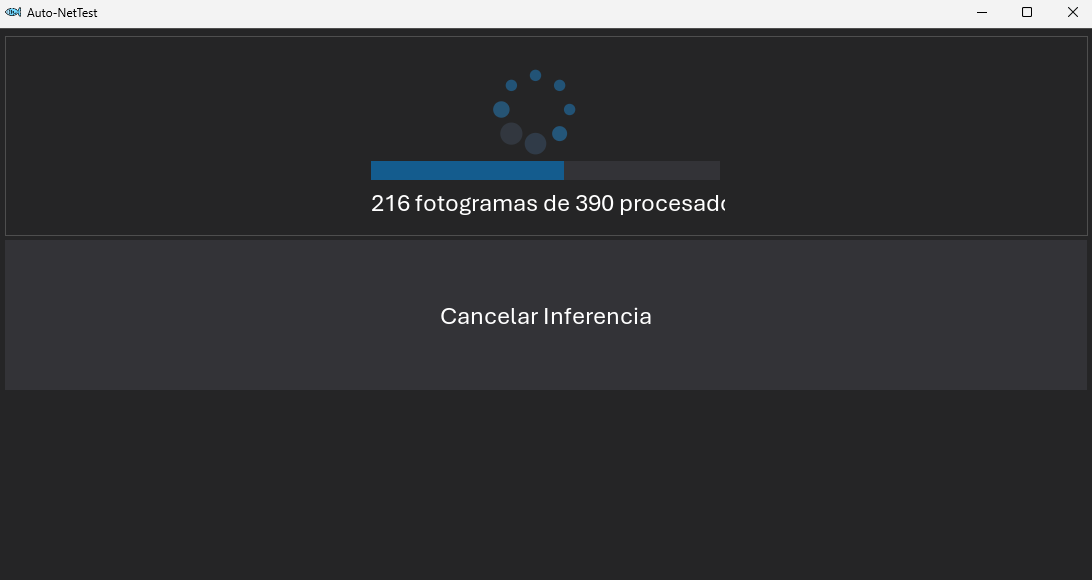
\includegraphics[width=0.7\textwidth]{images/9/CargaManual.png}
    \caption{Pantalla de carga en medio de un video con la barra de progreso}
    \label{fig:CargaParaManual}
\end{figure}

Finalizado el procesado del video, se pasa a la pantalla de guardado y análisis de resultados, cuyo aspecto y secciones se indican en la \autoref{fig:DatosManual}.

\begin{figure}[H]
    \centering
    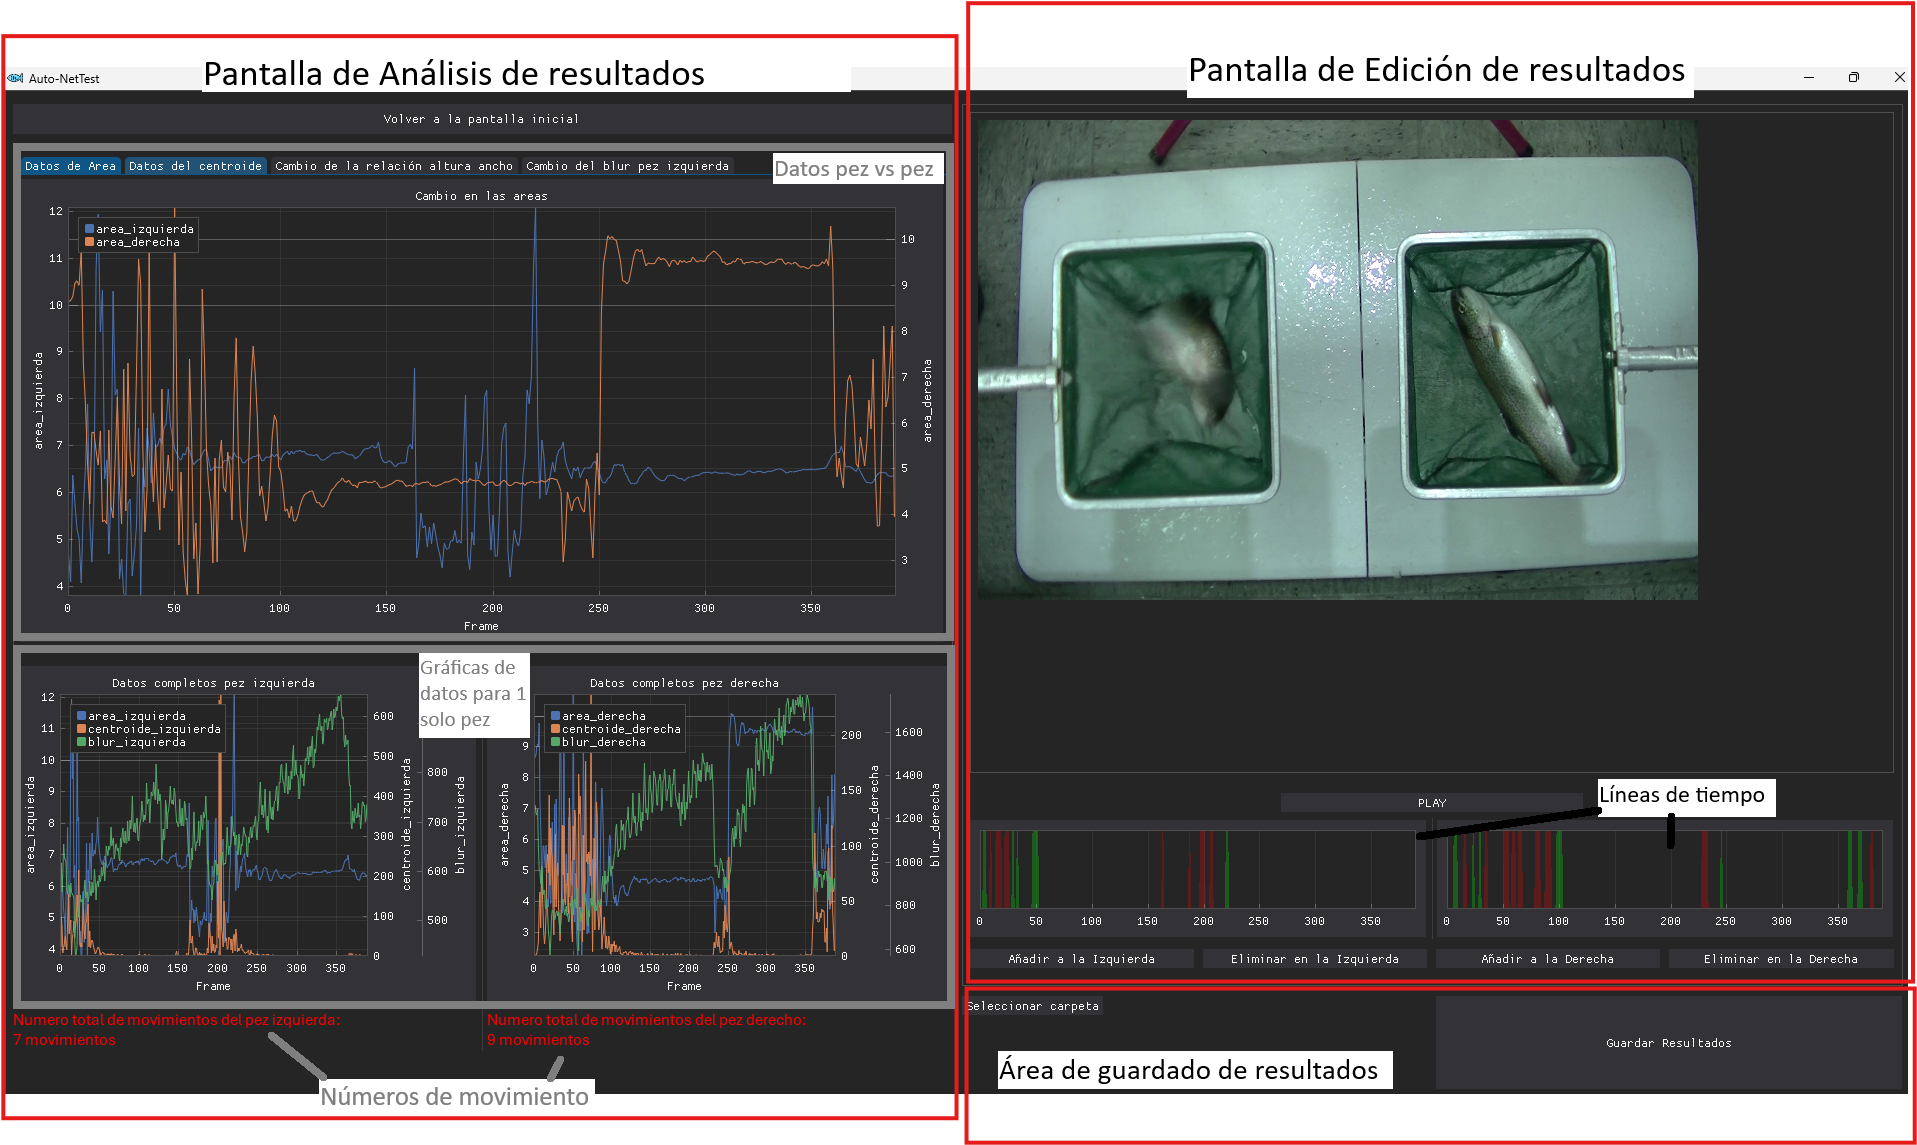
\includegraphics[width=\textwidth]{images/9/PantallaDatos.png}
    \caption{Pantalla de datos y sus zonas}
    \label{fig:DatosManual}
\end{figure}

Esta pantalla se divide en secciones, ya que cumple las funciones de muestra de datos obtenidos y de revisión/edición de los movimientos resultantes:
\begin{itemize}
    \item Sección de análisis de resultados: muestra los datos del área, centroide, relación de aspecto de la trucha y el \texttt{blur}, además del número de movimientos. En la parte vertical muestra para cada dato las dos gráficas 
    de las truchas para analizar comparativamente. En la parte inferior se muestran todos los datos para cada pez, de manera que se pueda hacer una correlación visual.
    \item Sección de edición y revisión de resultados: contiene un reproductor de video con una serie de controles y una pareja de líneas de tiempo. El reproductor funciona como se espera y la utilidad de las líneas de tiempo se 
    basa en la revisión y edición del número de movimientos que han ocurrido.

    En las líneas de tiempo, se marcan con rojo las situaciones en las que han ocurrido movimientos y en verde las situaciones en las que posiblemente hayan ocurrido movimientos, pero por ciertas reglas, no se han tenido en cuenta 
    y merecen ser revisadas manualmente (opcional).

    Las líneas de tiempo son seleccionables y, cuando se realiza un clic dentro de alguna de ellas el video se para y se deja una marca de la última posición en la que se ha clicado. Este comportamiento se puede observar en la 
    \autoref{fig:SeleccionMarcadoManual}, donde aparece un marcador azul.
    \begin{figure}[H]
        \centering
        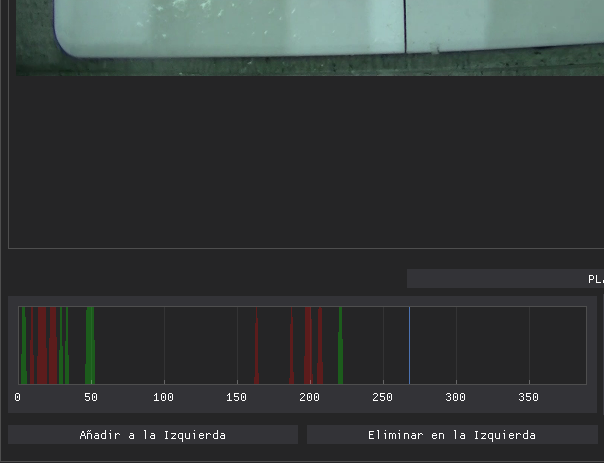
\includegraphics[width=0.8\textwidth]{images/9/Seleccion.png}
        \caption{Selección sobre una línea de tiempo y marcado}
        \label{fig:SeleccionMarcadoManual}
    \end{figure}
    Cuando se realiza este clic, el video se pausa y, la siguiente vez que se reproduzca, cambiará a esa posición. Además de esto, en esta posición podemos añadir o eliminar movimientos que hayan ocurrido como se ve en la \autoref{fig:AddManual}, 
    donde se añade un movimiento manualmente. Esto se verá reflejado en el número de movimientos que se marcan en la sección de análisis de resultados.
    \begin{figure}[H]
        \centering
        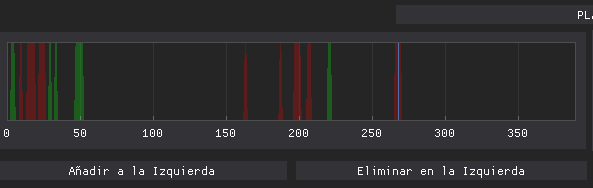
\includegraphics[width=0.5\textwidth]{images/9/Added.png}
        \caption{Movimiento añadido manualmente a través de la línea de tiempo}
        \label{fig:AddManual}
    \end{figure}

    \item Sección de guardado: contiene un simple explorador de carpetas para seleccionar un lugar donde guardar los archivos. Si no se selecciona ninguna carpeta, se guardan en el directorio donde se encuentre el ejecutable.\newline
    Se guardan los resultados en formato \texttt{CSV} y \texttt{JSON} para permitir flexibilidad e integrarlo en un procesado automático.
\end{itemize}

Finalmente, desde la pantalla de análisis de datos se puede volver a la pantalla inicial usando el botón correspondiente, que está situado en la parte superior izquierda.